\documentclass[conference]{IEEEtran}
\IEEEoverridecommandlockouts
\usepackage{cite}
\usepackage{amsmath,amssymb,amsfonts}
\usepackage{algorithmic}
\usepackage{graphicx}
\usepackage{textcomp}
\usepackage{subcaption}
\usepackage{xcolor}
\usepackage{booktabs}
\usepackage{url}
\def\BibTeX{{\rm B\kern-.05em{\sc i\kern-.025em b}\kern-.08em
    T\kern-.1667em\lower.7ex\hbox{E}\kern-.125emX}}

\begin{document}

\title{
The Application of Genetic Algorithms to the Bin Packing Problem \\
{\footnotesize \textnormal{ECM3412 - Nature-Inspired Computation}}
}

\author{\IEEEauthorblockN{Candidate Number: 730002704}
    \IEEEauthorblockA{\textit{University of Exeter} \\
        Exeter, United Kingdom \\
    }
}

\maketitle

\begin{abstract}
    This report investigates the application of genetic algorithms to the Bin Packing Problem, a classic optimisation problem. A literature review of nature-inspired algorithms for the BPP is presented, followed by an implementation of a genetic algorithm to solve two instances of the problem.
\end{abstract}

\begin{IEEEkeywords}
    genetic algorithms, bin-packing, optimisation, nature-inspired computation
\end{IEEEkeywords}

\textit{GenAI was not used in the completion of this coursework.}

\section{Introduction}
The Bin-Packing Problem (BPP) refers to the task of packing \(n\) items of varying weights into \(b\) bins such that the difference in weight between the heaviest and lightest bin is minimised \cite{delorme2018bpplib}.

Applications of the BPP range from table formatting to resource allocation \cite{johnson1974fast}.

In this report I investigate previous applications of nature-inspired algorithms to the BPP, implement a group of genetic algorithms to solve two instances of the BPP, and analyse the results obtained.

\section{Literature Review}
The Bin Packing Problem is an example of an NP-hard combinatorial problem \cite{dyckhoff1990typology}. As such, finding an optimal solution is infeasible for large instances, necessitating the use of heuristic approaches. In this literature review, I explore the use of nature-inspired algorithms for solving the BPP.

\subsection{Genetic Algorithm Variants}
To apply a standard genetic algorithm (GA) to the BPP, we need to choose a representation for candidate solutions. The most straightforward method is to use a list of integers, where the \(i\)-th integer represents the bin assigned to item \(i\). A weakness of this representation is that it creates a \textit{redundant search space}, where multiple genotypes map to the same phenotype. Consider that swapping all items between two bins does not change the solution, but results in a different genotype \cite{falkenauer1996hybrid}.

Falkenauer \cite{falkenauer1996hybrid} proposes using a \textit{grouping} representation, where the chromosome is a list of sets, each set representing the items in a bin. This eliminates redundancy but requires changing the operators used in the GA. Mutation involves either creating a new group, eliminating an existing group, or shuffling items amongst groups.

The performance of Falkenauer's grouping GA was evaluated against the MTP algorithm by Martello and Toth \cite{falkenauer1996hybrid}. They found that the genetic algorithm outperforms MTP on large problem instances, whilst still approaching optimal solutions.

\subsection{Particle Swarm Optimisation}
Particle Swarm Optimisation (PSO) is an algorithm inspired by the flocking behaviour of birds. Each `particle' in the swarm represents a candidate solution based on its position, and moves with some velocity determined by the algorithm. At each time step, each particle's velocity is updated to move it towards its own best-known position and the best-known position of the entire swarm. The weighting of these two influences is controlled by randomly generated coefficients \cite{omar2013solving}.

Omar and Ramakrishnan \cite{omar2013solving} enhanced the standard PSO algorithm with standard concepts from evolutionary algorithms, such as mutation and crossover, to create an `Evolutionary Particle Swarm Optimisation' (EPSO) algorithm. This algorithm was compared against a genetic algorithm (GA), simulated annealing (SA), and unified tabu search (UTS) on a set of benchmark BPP instances. They found that EPSO outperfomed GA and SA, and produced comparable results to UTS.

It is likely that the improved performance of PSO over GA is due to its utilisation of randomness to better explore the search space without getting caught in local optima. This reduces the premature convergence often seen in GAs.

\subsection{Ant Colony Optimisation}
The Ant Colony Optimisation (ACO) algorithm works well for combinatorial problems by simulating the path-finding behaviour of ants. It uses a `colony' of artificial ants that explore potential solutions. After an `ant' has constructed a solution, it deposits an amount of pheromone along the path taken proportional to the quality of the solution. This pheremone guides subsequent ants towards promising areas of the solution space \cite{dorigo1996ant}.

In order to solve the problem with ACO, we need to define two functions: the \textit{pheremone trail definition} and \textit{heuristic function}. The pheremone trail definition determines what is meant by the pheremone deposited by the ants. This is denoted \(\tau(i, j)\) for the pheremone level between items \(i\) and \(j\). This is defined to be the `favouribility' of having the two items in the same bin. The heuristic function, denoted \(\eta(i)\), defines the desirability of placing item \(i\) in the current bin. A simple heuristic function is to set \(\eta(i)\) to be the weight of item \(i\), so that heavier items are more likely to be placed in the current bin \cite{levine2004ant}.

From these definitions the standard application of ACO can be used to solve the BPP. Each ant iteratively constructs a solution by selecting items to place in the current bin based on the pheremone levels and heuristic values. A parameter \(\beta\) is used to control how much influence the heuristic function has on the selection process. Once an ant has filled a bin, it moves on to the next bin and continues until all items have been placed. After all ants have constructed their solutions, the pheremone levels are updated based on the quality of the solutions found \cite{levine2004ant}.

Levine and Ducatelle \cite{levine2004ant} found optimal parameters through experimentation. They found best results when the number of ants was equal to the number of items, whilst the rest of the parameters appeared not to be linked to features of the problem instance.

A weakness of this approach is its reliance on parameter tuning. This requires running the algorithm multiple times with different parameter settings to find the best configuration, which can be time-consuming. Since these parameters are based on specific problem instances, they will also not generalise well to other instances of the BPP.

\subsection{Other Nature-Inspired Approaches}
Simulated Annealing (SA) mimics the process of a solid slowly cooling until it freezes in a low-energy state. This is done by iteratively generating `neighbouring' solutions to the current candidate. This solution is always accepted if it is better than the current solution, but may sometimes be accepted even if it is worse, with probability \(e^{\frac{\delta}{T}}\), where \(\delta\) is the difference in fitness between the two solutions, and \(T\) is the current `temperature' which decreases over time \cite{bertsimas1993simulated}. Key parameters of the algorithm are the initial temperature, cooling rate, and stopping temperature.

Rao and Iyengar \cite{rao1994bin} applied simulated annealing to the same BPP variant that will be implemented later in this report. They found that, compared to the classic Largest Piece First (LPF), Smallest Piece First (SPF), and First Fit Decreasing (FFD) heuristics, SA produced better results with lower variance and more stabely across instances.

Tabu Search (TS) also iterates through neighbouring solutions, but maintains a \textit{tabu list} of recently visited solutions to avoid cycling back to them. The algorithm selects the best non-tabu neighbour at each iteration, allowing it to escape local optima \cite{glover1989tabu}.

Buljubašić and Vasquez \cite{buljubasic2016consistent} applied TS to the Bin Packing Problem. They initialised the algorithm with a complete solution generated by the First Fit heuristic on a random permutation of the items. Two solutions are considered neighbours if they differ by a single addition or removal of an item from a bin. This algorithm was compared to a GA and the BPP-specific algorithm `Perturbation-SAWMB'. They found that whilst all three algorithms could find the optimal solution for simpler instances, on more complex instances TS found significantly better solutions than the other two algorithms. Whilst Perturbation-SAWMB was slightly faster than TS, both were an order of magnitude slower than the GA.

A weakness of the TS approach is that it requires careful selection of the neighbourhood structure to be effective. A poorly chosen neighbourhood can lead to slow convergence or getting stuck in local optima. A method of generating initial solutions is also required. In general, TS also has a high number of tunable parameters that need to be optimised for each problem instance.

\subsection{Critical Analysis}
A common downside of all the genetic approaches is their reliance on parameter tuning. Whilst some, like PSO, have fewer parameters to tune, some like ACO and TS have many parameters that need to be optimised for each problem instance. This can lead to ineffective performance if the parameters are not well-chosen.

In all the literature, the genetic approaches outperform traditional heuristics like FFD and LPF. They are often able to find better solutions with lower variance across multiple runs. This is likely due to the nature of the problem having a large search space with many local optima, which nature-inspired algorithms are well-suited to explore.

A study which directly compares the different nature-inspired algorithms on a range of the same problem instances would be useful to determine which approach is most effective for the BPP, and which conditions favour each approach.

\section{Description of Results}
\subsection{Experimental Setup}
The parameters for the two Bin Packing Problems are given in Table \ref{tab:problems}. Table \ref{tab:params} gives the four configurations of parameters used in the genetic algorithm experiments.

Each configuration was run five times with different random seeds for 1,000 fitness evaluations. The best fitness, mean fitness, and standard deviation of fitness across the five runs were recorded, and the average fitness at each iteration was recorded for plotting.

\begin{table}[htbp]
    \caption{Description of Bin Packing Problems. The weight function \(\text{w}(i)\) gives the weight of item \(i\), where \(i \in [1, 500]\).}
    \begin{center}
        \begin{tabular}{|c|c|c|}
            \hline
            \textbf{Problem} & \textbf{Number of Bins} & \textbf{Weight Function}        \\
            \hline
            BPP1             & 10                      & \(\text{w}(i) = i\)             \\
            \hline
            BPP2             & 50                      & \(\text{w}(i) = \frac{i^2}{2}\) \\
            \hline
        \end{tabular}
        \label{tab:problems}
    \end{center}
\end{table}

\begin{table}[htbp]
    \centering
    \caption{The parameter values to be used.}
    \begin{tabular}{|c|c|c|c|c|}
        \hline
        \textbf{Parameter}    & \textbf{Conf. 1} & \textbf{Conf. 2} & \textbf{Conf. 3} & \textbf{Conf. 4} \\
        \hline
        Population Size \(p\) & 100              & 100              & 100              & 100              \\
        \hline
        Mutation Rate \(p_m\) & 0.01             & 0.05             & 0.01             & 0.05             \\
        \hline
        Tournament Size \(t\) & 3                & 3                & 7                & 7                \\
        \hline
    \end{tabular}
    \label{tab:params}
\end{table}

\subsection{Experimental Results}
\subsubsection{BPP1 Results (10 bins, 500 items)}
The results for BPP1 are summarised in Table \ref{tab:bpp1}, and the average fitness over iterations is shown in Figure \ref{fig:bpp1}.

\begin{table}[htbp]
    \caption{BPP1 Results Summary}
    \begin{center}
        \begin{tabular}{|c|c|c|c|c|}
            \hline
            \textbf{$p_m$} & \textbf{\(t\)} & \textbf{Best Fitness}   & \textbf{Mean Fitness}   & \textbf{Std. Dev}       \\
            \hline
            0.01           & 3              & \(7.84 \times 10^{-3}\) & \(7.32 \times 10^{-3}\) & \(2.03 \times 10^{-4}\) \\
            \hline
            0.05           & 3              & \(7.70 \times 10^{-3}\) & \(6.76 \times 10^{-3}\) & \(3.87 \times 10^{-4}\) \\
            \hline
            0.01           & 7              & \(7.90 \times 10^{-3}\) & \(7.59 \times 10^{-3}\) & \(1.25 \times 10^{-4}\) \\
            \hline
            0.05           & 7              & \(7.73 \times 10^{-3}\) & \(7.10 \times 10^{-3}\) & \(2.75 \times 10^{-4}\) \\
            \hline
        \end{tabular}
        \label{tab:bpp1}
    \end{center}
\end{table}


\subsubsection{BPP2 Results (50 bins, 500 items)}
The results for BPP2 are summarised in Table \ref{tab:bpp2}, and the average fitness over iterations is shown in Figure \ref{fig:bpp2}.

\begin{table}[htbp]
    \caption{BPP2 Results Summary}
    \begin{center}
        \begin{tabular}{|c|c|c|c|c|}
            \hline
            \textbf{$p_m$} & \textbf{\(t\)} & \textbf{Best Fitness}   & \textbf{Mean Fitness}   & \textbf{Std Dev}        \\
            \hline
            0.01           & 3              & \(1.96 \times 10^{-4}\) & \(1.69 \times 10^{-4}\) & \(1.14 \times 10^{-5}\) \\
            \hline
            0.05           & 3              & \(1.75 \times 10^{-4}\) & \(1.34 \times 10^{-4}\) & \(1.20 \times 10^{-5}\) \\
            \hline
            0.01           & 7              & \(2.01 \times 10^{-4}\) & \(1.83 \times 10^{-4}\) & \(1.19 \times 10^{-5}\) \\
            \hline
            0.05           & 7              & \(1.83 \times 10^{-4}\) & \(1.49 \times 10^{-4}\) & \(1.30 \times 10^{-5}\) \\
            \hline
        \end{tabular}
        \label{tab:bpp2}
    \end{center}
\end{table}

\section{Discussion and Further Work}

\subsection{Question 1: Which combination of parameters produces the best results?}
In both instances, the configuration with \(p_m=0.01\) and \(t=7\) led to the highest mean and best fitness values, as can be seen in Tables \ref{tab:bpp1} and \ref{tab:bpp2}. The standard deviation for this configuration was also the lowest for DPP1, and second lowest for DPP2, indicating more consistent performance.

\subsection{Question 2: What do you think is the reason for your findings in Question 1?}
A lower mutation rate helps to preserve beneficial traits in the population. A larger tournament size increases selection pressure, favouring fitter individuals. Decreasing the mutation rate too far would limit how much the population could explore the search space over the limited iterations, while increasing the tournament size too much would lead to premature convergence.

\subsection{Question 3: How do each of the parameter settings influence the performance of the algorithm?}
By comparing the groups of graphs for each instance given in Figures \ref{fig:bpp1} and \ref{fig:bpp2}, we can see the effects of changing each parameter:
\begin{itemize}
    \item \(p_m = 0.01\) always leads to a higher mean fitness than \(p_m = 0.05\). This is likely because a lower mutation rate helps to preserve beneficial traits in the population.
    \item At \(t=7\) the population converges more quickly than at \(t=3\). Note how much steeper the initial fitness increase is in \ref{fig:bpp1} (c) compared to (a), and similarly in \ref{fig:bpp2}. This is because a larger tournament size increases selection pressure, favouring fitter individuals and reducing the survival of less fit individuals.
    \item In the first instance, BPP1, setting \(t=7\) leads to a lower (by around \(40\%\)) standard deviation than \(t=3\), indicating more consistent performance. In BPP2 there is a slight increase. This may be because the larger search space of BPP2 may lead to premature convergence when using a larger tournament size.
\end{itemize}

\subsection{Question 4: Do you think that one of the algorithms in your literature review might have provided better results? Explain your answer.}
From the literature review, it seems that Ant Colony Optimisation (ACO) and Evolutionary Particle Swarm Optimisation (EPSO) have both been shown to outperform genetic algorithms on the Bin Packing Problem \cite{levine2004ant, omar2013solving}. These algorithms are better at avoiding local optima due to their increased diversity in the population.

ACO uses pheromone trails to guide the search towards promising areas of the solution space, while EPSO uses velocity updates. Both of these mechanisms maintain the diversity of the population better than standard genetic algorithms, which can suffer from premature convergence due to selection pressure and loss of genetic diversity.

\subsection{Further Experiments}
My first experiment was into the role of population size on the performance of the algorithm. Using BPP2 with \(p_m=0.01\) and \(t=7\), I ran the algorithm with population sizes of 10, 50, 100, 400, and 800 for three trials each. The results are shown in Figure \ref{fig:population_size_experiment}. The number of iterations was fixed, so the number of fitness evaluations increased with population size.

I found that increasing the population size tended to decrease the average fitness. This could be due to the search space being able to be explored with only a few individuals, and so a small population can more efficiently find good solutions. Over higher iterations and with different parameters, a large population could be more beneficial to maintain diversity.

\begin{figure}[htbp]
    \centering
    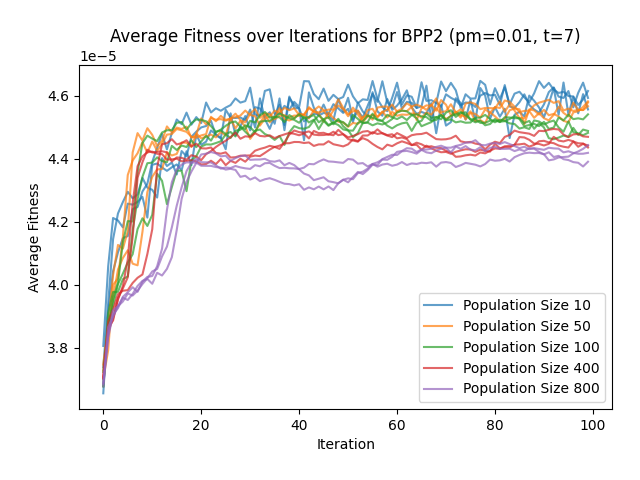
\includegraphics[width=\linewidth]{bpp_ga_population_size_experiment.png}
    \caption{Effect of Population Size on Average Fitness over Iterations for BPP2 with \(p_m=0.01\) and \(t=7\).}
    \label{fig:population_size_experiment}
\end{figure}

The second experiment varied the mutation rate more widely, using values of 0.0001, 0.001, 0.01, 0.1, and 1.0, with \(p=100\) and \(t=7\) on BPP2. Each configuration was run three times. The results are shown in Figure \ref{fig:mutation_rate_experiment}.

The best performance was achieved with \(p_m=0.001\). The performance of \(p_m=0.0001\) was slightly lower, likely because the mutation rate was too low to explore the search space effectively. Higher mutation rates led to significantly worse performance, as excessive mutation disrupts beneficial traits in the population. At \(p_m=1.0\), the algorithm cannot retain any beneficial traits, leading to random search behaviour.

\begin{figure}[htbp]
    \centering
    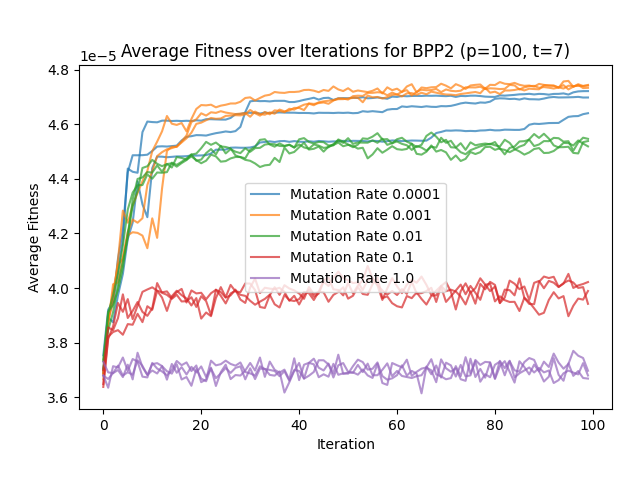
\includegraphics[width=\linewidth]{bpp_ga_mutation_rate_experiment.png}
    \caption{Effect of Mutation Rate on Average Fitness over Iterations for BPP2 with \(p=100\) and \(t=7\).}
    \label{fig:mutation_rate_experiment}
\end{figure}

\subsection{Future Work}
It would be interesting to explore the effects of modifying the parameters over the course of the algorithm's execution, such as using a higher mutation rate in early generations to encourage exploration, and lowering it later to refine solutions.

A different encoding with less redundancy could be investigated, for instance the grouping representation proposed by Falkenauer \cite{falkenauer1996hybrid}. This would require custom operators and a more complex implementation to deal with the encoding scheme, but could potentially yield better results.

\section{Conclusion}
In this report I have implemented a GA to solve two instances of the BPP. The results indicate that a lower mutation rate and larger tournament size improve the algorithm's performance.

From the results, we can see that the instances converge more quickly on BPP1 and on a fitter solution than BPP2, likely due to the smaller search space. The best configurations also result in a low standard deviation, indicating consistent performance.

My further experiments into population size and mutation rate show that smaller populations and lower mutation rates tend to yield better results, although there is a balance to be struck to maintain diversity.

\begin{figure*}[htbp]
    \centering
    \caption{BPP1 Results. Note that the axis scales are consistent across the subfigures.}

    \begin{subfigure}{0.7\linewidth}
        \centering
        \begin{minipage}{0.48\linewidth}
            \centering
            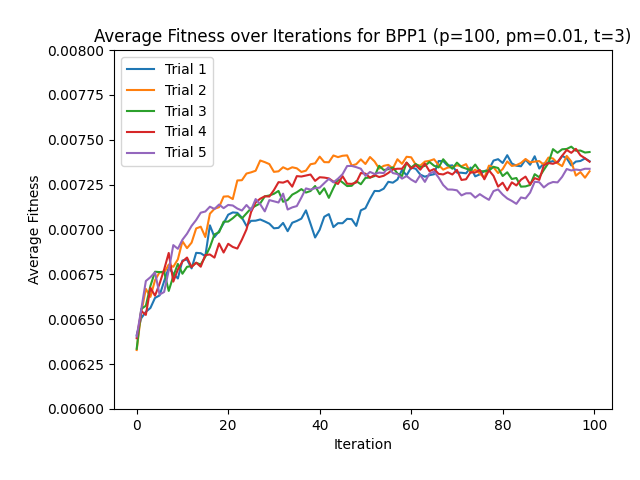
\includegraphics[width=\linewidth]{bpp_ga_results_BPP1_p100_pm0.01_t3.png}
            \caption*{(a) $p_m = 0.01$, $t = 3$}
        \end{minipage}\hfill
        \begin{minipage}{0.48\linewidth}
            \centering
            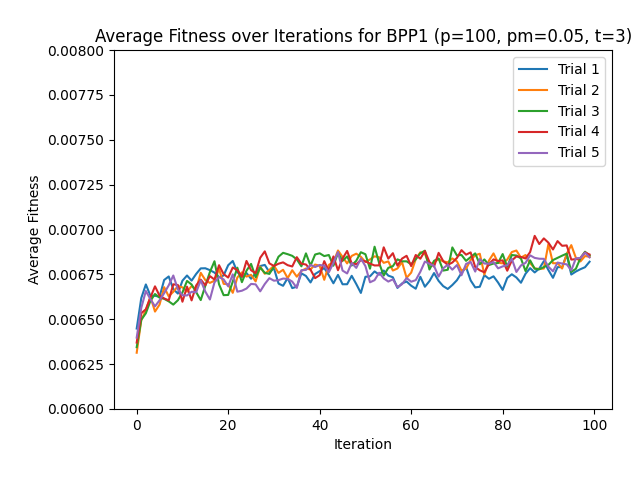
\includegraphics[width=\linewidth]{bpp_ga_results_BPP1_p100_pm0.05_t3.png}
            \caption*{(b) $p_m = 0.05$, $t = 3$}
        \end{minipage}
    \end{subfigure}

    \begin{subfigure}{0.7\linewidth}
        \centering
        \begin{minipage}{0.48\linewidth}
            \centering
            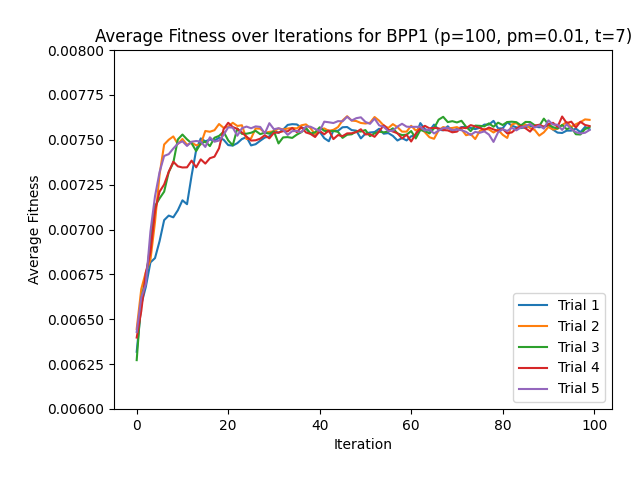
\includegraphics[width=\linewidth]{bpp_ga_results_BPP1_p100_pm0.01_t7.png}
            \caption*{(c) $p_m = 0.01$, $t = 7$}
        \end{minipage}\hfill
        \begin{minipage}{0.48\linewidth}
            \centering
            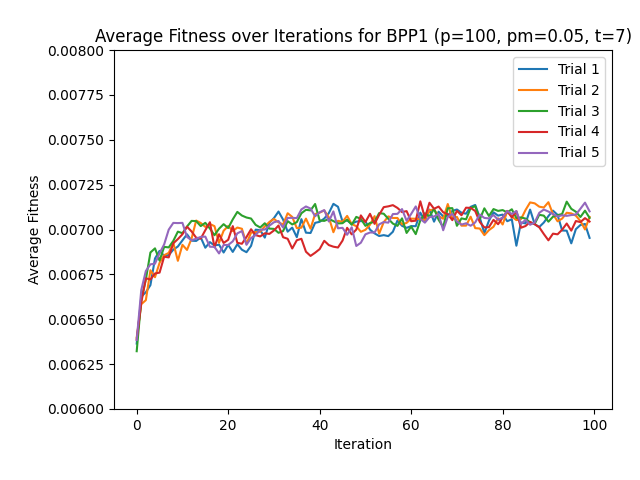
\includegraphics[width=\linewidth]{bpp_ga_results_BPP1_p100_pm0.05_t7.png}
            \caption*{(d) $p_m = 0.05$, $t = 7$}
        \end{minipage}
    \end{subfigure}

    \label{fig:bpp1}
\end{figure*}

\begin{figure*}[htbp]
    \centering
    \caption{BPP2 Results. Note that the axis scales differ from those in Figure \ref{fig:bpp1} but are consistent across the subfigures here.}

    \begin{subfigure}{0.7\linewidth}
        \centering
        \begin{minipage}{0.48\linewidth}
            \centering
            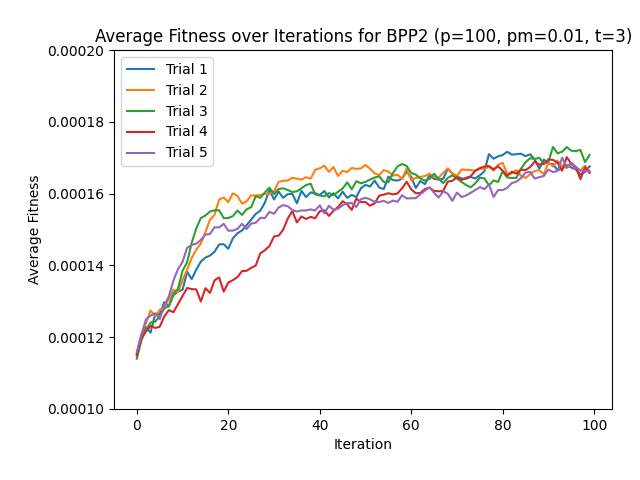
\includegraphics[width=\linewidth]{bpp_ga_results_BPP2_p100_pm0.01_t3.png}
            \caption*{(a) $p_m = 0.01$, $t = 3$}
        \end{minipage}\hfill
        \begin{minipage}{0.48\linewidth}
            \centering
            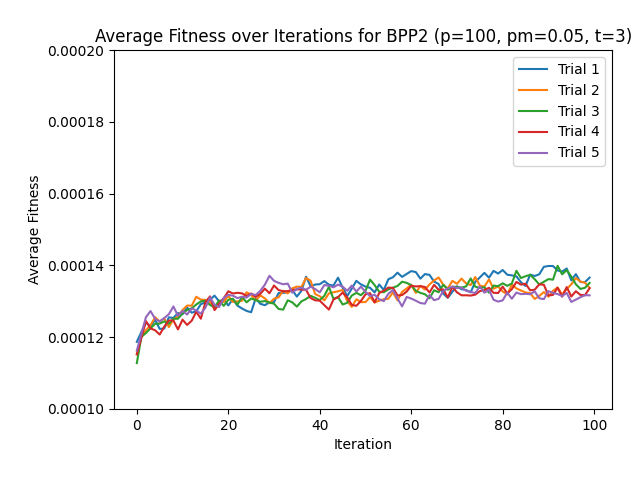
\includegraphics[width=\linewidth]{bpp_ga_results_BPP2_p100_pm0.05_t3.png}
            \caption*{(b) $p_m = 0.05$, $t = 3$}
        \end{minipage}
    \end{subfigure}

    \begin{subfigure}{0.7\linewidth}
        \centering
        \begin{minipage}{0.48\linewidth}
            \centering
            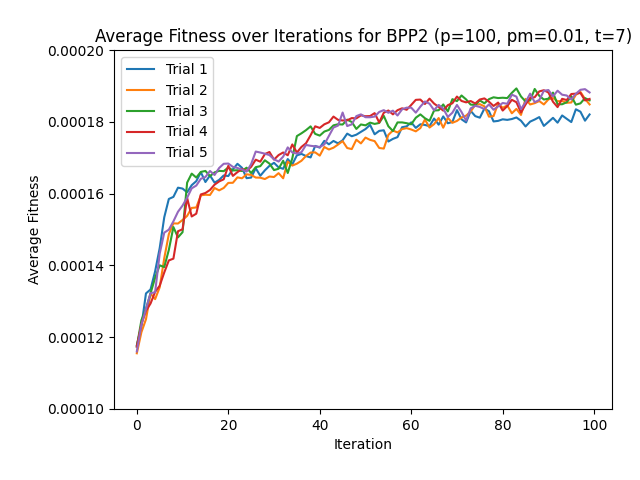
\includegraphics[width=\linewidth]{bpp_ga_results_BPP2_p100_pm0.01_t7.png}
            \caption*{(c) $p_m = 0.01$, $t = 7$}
        \end{minipage}\hfill
        \begin{minipage}{0.48\linewidth}
            \centering
            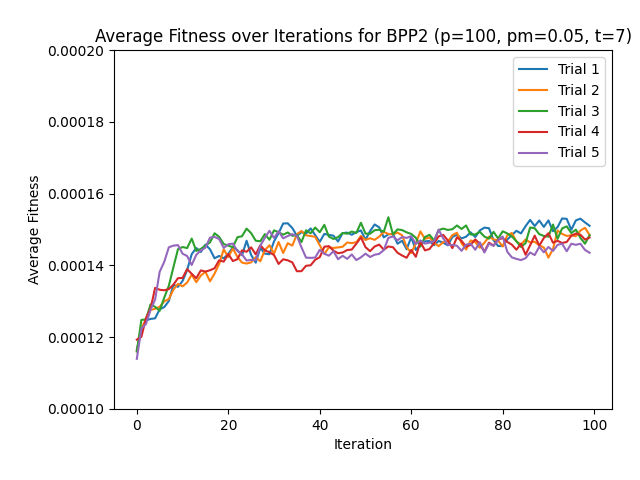
\includegraphics[width=\linewidth]{bpp_ga_results_BPP2_p100_pm0.05_t7.png}
            \caption*{(d) $p_m = 0.05$, $t = 7$}
        \end{minipage}
    \end{subfigure}

    \label{fig:bpp2}
\end{figure*}

\begin{thebibliography}{00}
    \bibitem{falkenauer1996hybrid} E. Falkenauer, ``A hybrid grouping genetic algorithm for bin packing,'' J Heuristics, vol. 2, no. 1, pp. 5–30, 1996, doi: 10.1007/BF00226291.
    \bibitem{delorme2018bpplib} M. Delorme, M. Iori, and S. Martello, ``BPPLIB: a library for bin packing and cutting stock problems,'' Optim Lett, vol. 12, no. 2, pp. 235–250, Mar. 2018, doi: 10.1007/s11590-017-1192-z.
    \bibitem{johnson1974fast} D. S. Johnson, ``Fast algorithms for bin packing,'' Journal of Computer and System Sciences, vol. 8, no. 3, pp. 272–314, Jun. 1974, doi: 10.1016/S0022-0000(74)80026-7.
    \bibitem{dyckhoff1990typology} H. Dyckhoff, ``A typology of cutting and packing problems,'' European Journal of Operational Research, vol. 44, no. 2, pp. 145–159, Jan. 1990, doi: 10.1016/0377-2217(90)90350-K.
    \bibitem{dorigo1996ant} M. Dorigo, V. Maniezzo, and A. Colorni, ``Ant system: optimization by a colony of cooperating agents,'' IEEE Trans. Syst., Man, Cybern. B, vol. 26, no. 1, pp. 29–41, Feb. 1996, doi: 10.1109/3477.484436.
    \bibitem{levine2004ant} J. Levine and F. Ducatelle, ``Ant colony optimization and local search for bin packing and cutting stock problems,'' Journal of the Operational Research Society, vol. 55, no. 7, pp. 705–716, Jul. 2004, doi: 10.1057/palgrave.jors.2601771.
    \bibitem{omar2013solving} M. K. Omar and K. Ramakrishnan, ``Solving non-oriented two dimensional bin packing problem using evolutionary particle swarm optimisation,'' International Journal of Production Research, vol. 51, no. 20, pp. 6002–6016, Oct. 2013, doi: 10.1080/00207543.2013.791754.
    \bibitem{bertsimas1993simulated} D. Bertsimas and J. Tsitsiklis, ``Simulated Annealing,'' Statist. Sci., vol. 8, no. 1, Feb. 1993, doi: 10.1214/ss/1177011077.
    \bibitem{rao1994bin} R. L. Rao and S. S. Iyengar, ``Bin-packing by simulated annealing,'' Computers \& Mathematics with Applications, vol. 27, no. 5, pp. 71–82, Mar. 1994, doi: 10.1016/0898-1221(94)90077-9.
    \bibitem{glover1989tabu} F. Glover and M. Laguna, Tabu Search. Boston, MA: Springer US, 1997. doi: 10.1007/978-1-4615-6089-0.
    \bibitem{buljubasic2016consistent} M. Buljubašić and M. Vasquez, ``Consistent neighborhood search for one-dimensional bin packing and two-dimensional vector packing,'' Computers \& Operations Research, vol. 76, pp. 12–21, Dec. 2016, doi: 10.1016/j.cor.2016.06.009.
\end{thebibliography}

\end{document}
